\section{Auswertung}
\subsection{Ermitteln des Brechungsindex einer Glasprobe}
	Nach der in Abschnitt (\ref{sec:shimadzu}) beschriebenen Messung des spektralen Transmissions- und Reflexionsvermögens im Wellenlängenbereich von $\lambda = 250\dots800\ \unit{nm}$ ergeben sich die in Abbildung \ref{fig:R_T_glas} dargestellten Spektren.
	\begin{figure}[ht]
		\centering
		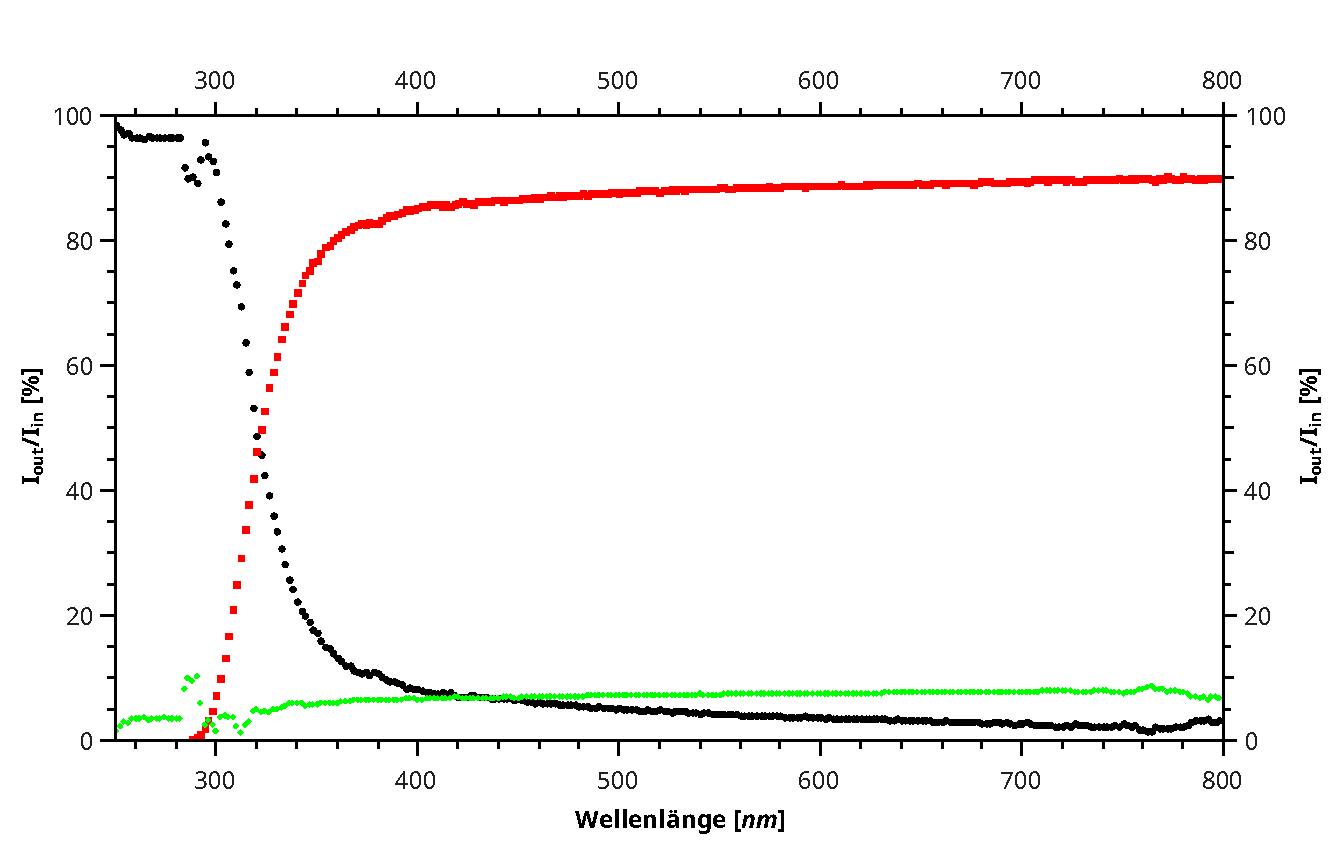
\includegraphics[width=\linewidth]{pic/R_T_glas.pdf}
		\caption{Spektrales Transmissions- (rot), Reflexions- (grün) und Absorptionsvermögen (schwarz) einer Glasprobe}
		\label{fig:R_T_glas}
	\end{figure}
	Dabei wurde angenommen, dass das Absorptionsvermögen durch $A = 1 - R - T$ gegeben ist. Man sieht deutlich, dass das Glas wie ein Kantenfilter wirkt, welcher elektromagnetische Wellen unterhalb einer Wellenlänge von $\unit[300]{nm}$ absorbiert. Im sichtbaren Bereich von etwa 400 bis $\unit[800]{nm}$ ist das Glas hauptsächlich transparent, da das Transmissionsvermögen etwa $\unit[90]{\%}$ beträgt.\\
	Mit Hilfe der Formeln (\ref{eq:n_T}) und (\ref{eq:n_R}) kann aus dem Spektrum der wellenlängenabhängige Brechungsindex bestimmt werden. Abbildung \ref{fig:n_glas} zeigt den Verlauf für die Berechnung aus dem Transmissions- und dem Reflexionsvermögen.
	\begin{figure} [ht]
				\centering
				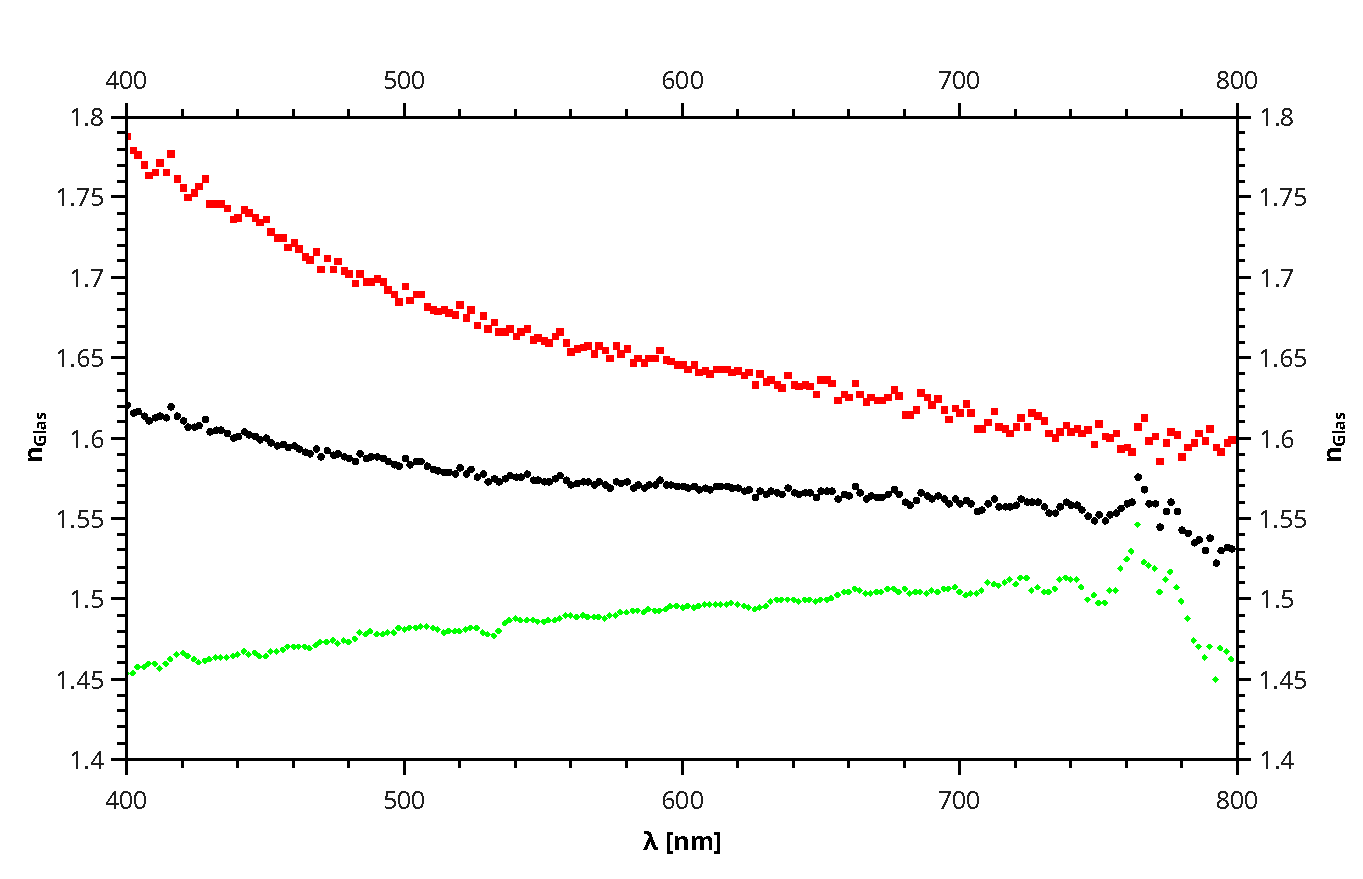
\includegraphics[width=\linewidth]{pic/n_glas.pdf}
				\caption{Wellenlängenabhängiger Brechungsindex. Dieser wurde aus dem Transmissionsvermögen (rot), dem Reflexionsvermögen (grün) bestimmt und anschließend gemittelt (schwarz).}
				\label{fig:n_glas}
	\end{figure} 
	Beide Berechnungen sollten theoretisch zu einem identischen Ergebnis führen, was offensichtlich nicht der Fall ist. Ein möglicher Grund dafür ist die Tatsache, dass Absorption im Medium stattfindet und somit die Relation $1 = T_{ges} + R_{ges}$, die in der Herleitung aus Abschnitt (\ref{sec:fresnel}) verwendet wurde, nicht gültig ist. Da die Absorption allerdings schwach im Vergleich zur Transmission ist, ist die obige Herleitung eine akzeptable Näherung. Mittelt man beide errechnete Werte, erhält man den erwarteten Verlauf, dass der Brechungsindex im sichtbaren Bereich für große Wellenlängen immer weiter abnimmt. Dieser Effekt wird \textit{Dispersion} genannt und er erklärt die spektrale Aufspaltung von Licht, die beispielsweise an einem Glasprisma auftritt.Mittelt man über den gesamten sichtbaren Wellenlängenbereich erhält man einen mittleren Brechungsindex für den vorliegenden Glasfilter von:
	\begin{equation}
		\bar{n} = 1,57 \pm 0,02.
	\end{equation}
	Hierbei steht die Fehlerangabe für die Standardabweichung der aufgenommenen Messpunkte um den Mittelwert.\\
	Für Wellenlängen unterhalb  von $\unit[400]{nm}$ ist es nicht sinnvoll den Brechungsindex mit der oben angegebenen Methode zu berechnen, da Absorptionseffekte immer signifikanter werden. Um dies noch besser zu berücksichtigen müsste man den Brechungsindex als komplexe Größe auffassen, d.h. $n \rightarrow N := n(1 + \kappa) \in \mathbb{C}$.
	